\documentclass{standalone}

\usepackage{bm}
\usepackage{fontspec}
\usepackage{tikz}

\usetikzlibrary{arrows.meta}
\usetikzlibrary{backgrounds}
\usetikzlibrary{fit}
\usetikzlibrary{matrix}
\usetikzlibrary{positioning}
\usetikzlibrary{shapes.geometric}

\newcommand{\mat}[1]{\bm{#1}}
\newcommand{\Tr}{^{\top}}
\newcommand{\vc}[1]{\bm{#1}}

\setmainfont{Liberation Sans}
\newlength{\mywidth}
\newlength{\myheight}

\makeatletter
\DeclareRobustCommand{\rvdots}{%
  \vbox{
    \baselineskip4\p@\lineskiplimit\z@
    \kern-\p@
    \hbox{.}\hbox{.}\hbox{.}
  }}
\makeatother

\begin{document}
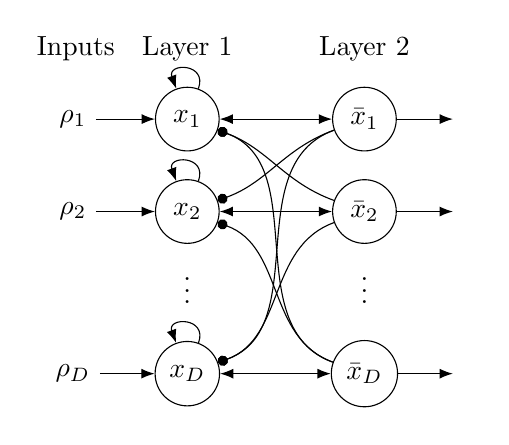
\begin{tikzpicture}[
    every path/.style={-{Latex}},
    inhibit/.style={-{Circle}},
    neuron/.style={circle, minimum size=23, draw=black},
    gate/.style={diamond, draw=black},
    net/.style={rectangle, draw=black},
    ]

    \matrix [column sep=20, row sep=10] {
        \node (rho1) {$\rho_1$}; & \node (x1) [neuron] {$x_1$}; &[20] \node 
        (bar-x1) [neuron] {$\bar{x}_1$}; & \node (out1) {}; \\
        \node (rho2) {$\rho_2$}; & \node (x2) [neuron] {$x_2$}; & \node (bar-x2) 
        [neuron] [neuron] {$\bar{x}_2$}; & \node (out2) {}; \\
        & \node {$\rvdots$}; & \node {$\rvdots$}; & \\
        \node (rhoD) {$\rho_D$}; & \node (xD) [neuron] {$x_D$}; & \node (bar-xD) 
        [neuron] {$\bar{x}_D$}; & \node (outD) {}; \\
    };

    \foreach \i in {1, 2, D} {
        \draw [loop above, min distance=10, in=110, out=70] (x\i) to (x\i);
        \draw (rho\i) to (x\i);
        \draw (x\i) [{Latex}-{Latex}] to  (bar-x\i);
        \draw (bar-x\i) to (out\i);
    }
    \foreach \i/\j in {1/2, 1/D, 2/D} {
        \draw (bar-x\i) [inhibit, in=20, out=200]  to (x\j);
    }
    \foreach \i/\j in {2/1, D/1, D/2} {
        \draw (bar-x\i) [inhibit, in=-20, out=160]  to (x\j);
    }

    \node (l1) [above=0.2cm of x1] {Layer 1};
    \node [above=0.2cm of bar-x1] {Layer 2};
    \node [left=0.1cm of l1] {Inputs};
\end{tikzpicture}
\end{document}
